\documentclass[1p]{elsarticle_modified}
%\bibliographystyle{elsarticle-num}

%\usepackage[colorlinks]{hyperref}
%\usepackage{abbrmath_seonhwa} %\Abb, \Ascr, \Acal ,\Abf, \Afrak
\usepackage{amsfonts}
\usepackage{amssymb}
\usepackage{amsmath}
\usepackage{amsthm}
\usepackage{scalefnt}
\usepackage{amsbsy}
\usepackage{kotex}
\usepackage{caption}
\usepackage{subfig}
\usepackage{color}
\usepackage{graphicx}
\usepackage{xcolor} %% white, black, red, green, blue, cyan, magenta, yellow
\usepackage{float}
\usepackage{setspace}
\usepackage{hyperref}

\usepackage{tikz}
\usetikzlibrary{arrows}

\usepackage{multirow}
\usepackage{array} % fixed length table
\usepackage{hhline}

%%%%%%%%%%%%%%%%%%%%%
\makeatletter
\renewcommand*\env@matrix[1][\arraystretch]{%
	\edef\arraystretch{#1}%
	\hskip -\arraycolsep
	\let\@ifnextchar\new@ifnextchar
	\array{*\c@MaxMatrixCols c}}
\makeatother %https://tex.stackexchange.com/questions/14071/how-can-i-increase-the-line-spacing-in-a-matrix
%%%%%%%%%%%%%%%

\usepackage[normalem]{ulem}

\newcommand{\msout}[1]{\ifmmode\text{\sout{\ensuremath{#1}}}\else\sout{#1}\fi}
%SOURCE: \msout is \stkout macro in https://tex.stackexchange.com/questions/20609/strikeout-in-math-mode

\newcommand{\cancel}[1]{
	\ifmmode
	{\color{red}\msout{#1}}
	\else
	{\color{red}\sout{#1}}
	\fi
}

\newcommand{\add}[1]{
	{\color{blue}\uwave{#1}}
}

\newcommand{\replace}[2]{
	\ifmmode
	{\color{red}\msout{#1}}{\color{blue}\uwave{#2}}
	\else
	{\color{red}\sout{#1}}{\color{blue}\uwave{#2}}
	\fi
}

\newcommand{\Sol}{\mathcal{S}} %segment
\newcommand{\D}{D} %diagram
\newcommand{\A}{\mathcal{A}} %arc


%%%%%%%%%%%%%%%%%%%%%%%%%%%%%5 test

\def\sl{\operatorname{\textup{SL}}(2,\Cbb)}
\def\psl{\operatorname{\textup{PSL}}(2,\Cbb)}
\def\quan{\mkern 1mu \triangleright \mkern 1mu}

\theoremstyle{definition}
\newtheorem{thm}{Theorem}[section]
\newtheorem{prop}[thm]{Proposition}
\newtheorem{lem}[thm]{Lemma}
\newtheorem{ques}[thm]{Question}
\newtheorem{cor}[thm]{Corollary}
\newtheorem{defn}[thm]{Definition}
\newtheorem{exam}[thm]{Example}
\newtheorem{rmk}[thm]{Remark}
\newtheorem{alg}[thm]{Algorithm}

\newcommand{\I}{\sqrt{-1}}
\begin{document}

%\begin{frontmatter}
%
%\title{Boundary parabolic representations of knots up to 8 crossings}
%
%%% Group authors per affiliation:
%\author{Yunhi Cho} 
%\address{Department of Mathematics, University of Seoul, Seoul, Korea}
%\ead{yhcho@uos.ac.kr}
%
%
%\author{Seonhwa Kim} %\fnref{s_kim}}
%\address{Center for Geometry and Physics, Institute for Basic Science, Pohang, 37673, Korea}
%\ead{ryeona17@ibs.re.kr}
%
%\author{Hyuk Kim}
%\address{Department of Mathematical Sciences, Seoul National University, Seoul 08826, Korea}
%\ead{hyukkim@snu.ac.kr}
%
%\author{Seokbeom Yoon}
%\address{Department of Mathematical Sciences, Seoul National University, Seoul, 08826,  Korea}
%\ead{sbyoon15@snu.ac.kr}
%
%\begin{abstract}
%We find all boundary parabolic representation of knots up to 8 crossings.
%
%\end{abstract}
%\begin{keyword}
%    \MSC[2010] 57M25 
%\end{keyword}
%
%\end{frontmatter}

%\linenumbers
%\tableofcontents
%
\newcommand\colored[1]{\textcolor{white}{\rule[-0.35ex]{0.8em}{1.4ex}}\kern-0.8em\color{red} #1}%
%\newcommand\colored[1]{\textcolor{white}{ #1}\kern-2.17ex	\textcolor{white}{ #1}\kern-1.81ex	\textcolor{white}{ #1}\kern-2.15ex\color{red}#1	}

{\Large $\underline{12a_{0071}~(K12a_{0071})}$}

\setlength{\tabcolsep}{10pt}
\renewcommand{\arraystretch}{1.6}
\vspace{1cm}\begin{tabular}{m{100pt}>{\centering\arraybackslash}m{274pt}}
\multirow{5}{120pt}{
	\centering
	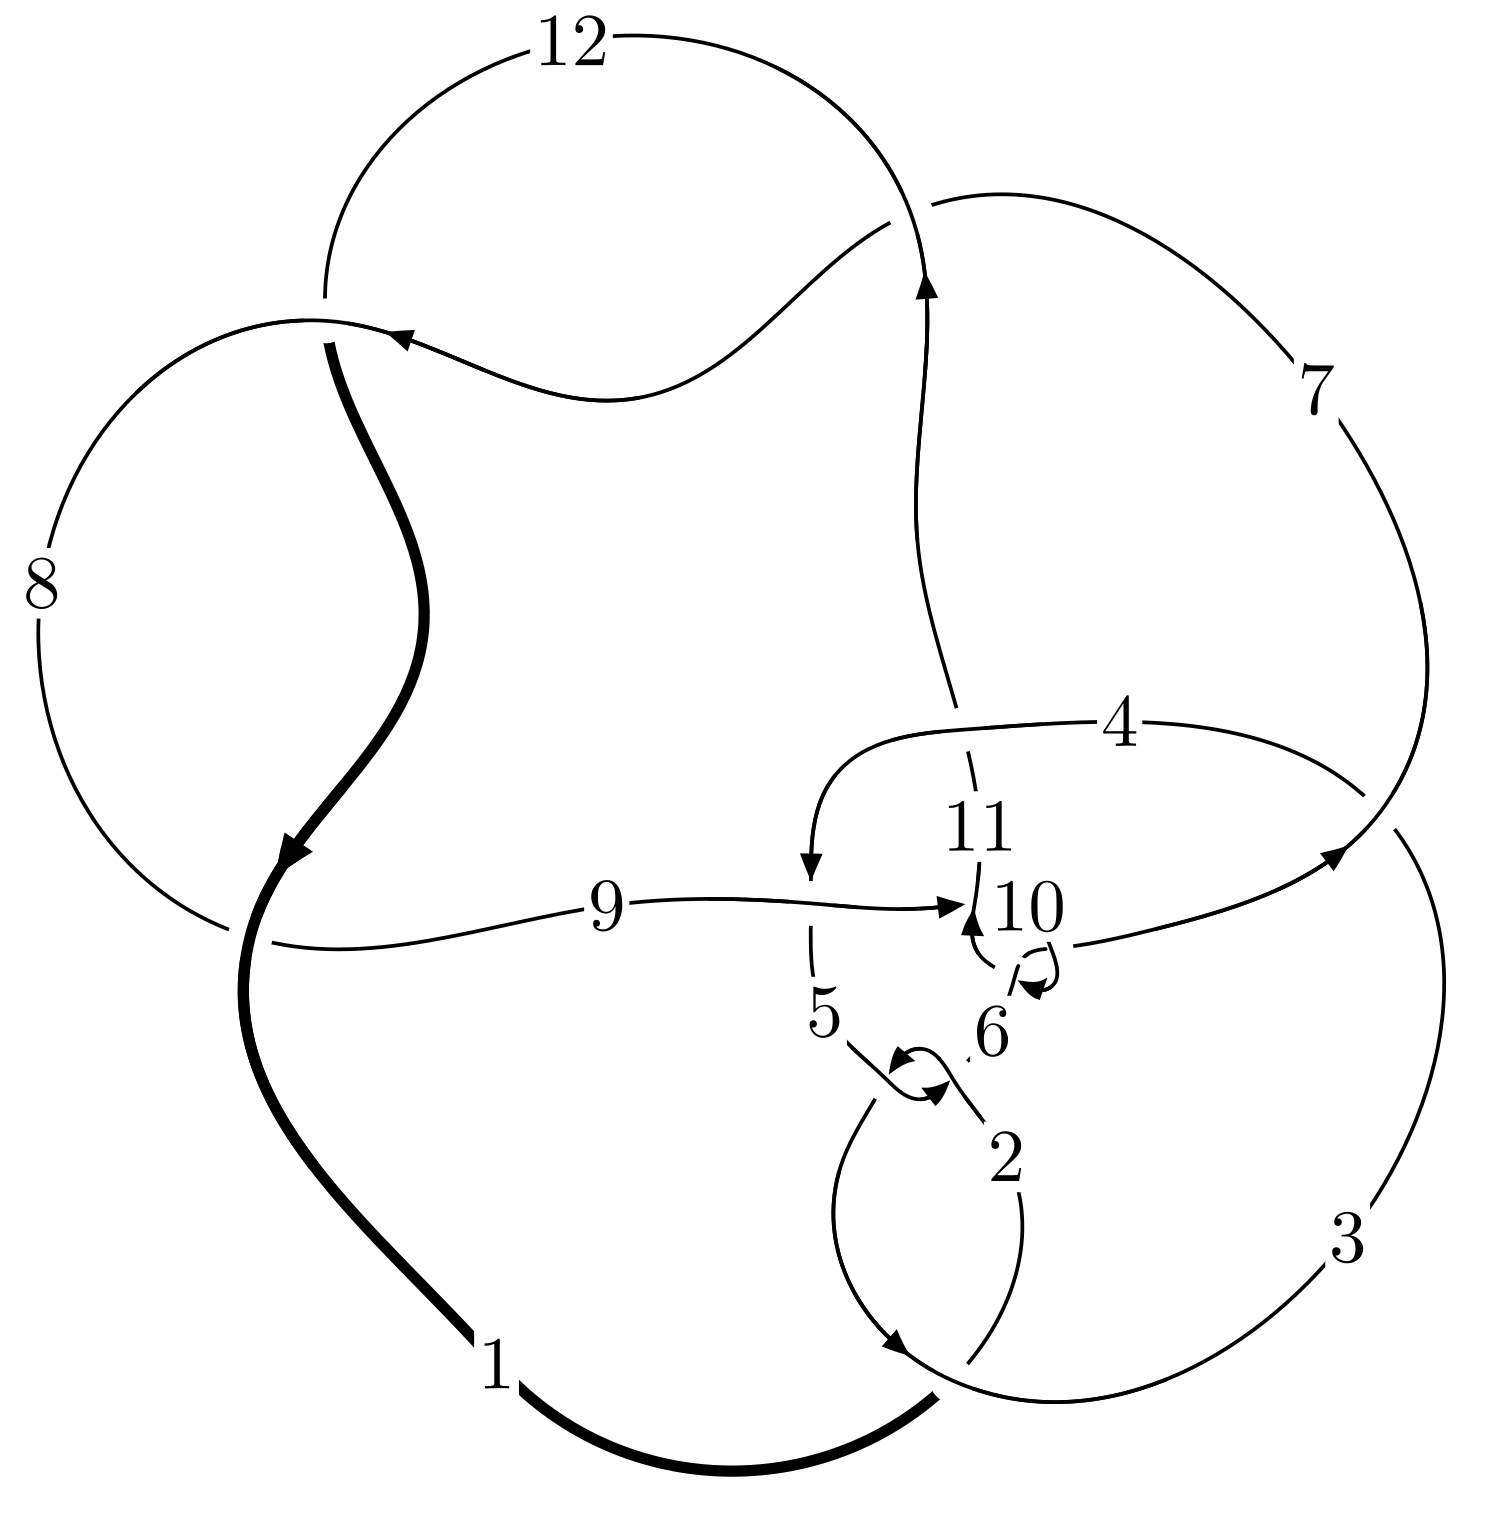
\includegraphics[width=112pt]{../../../GIT/diagram.site/Diagrams/png/872_12a_0071.png}\\
\ \ \ A knot diagram\footnotemark}&
\allowdisplaybreaks
\textbf{Linearized knot diagam} \\
\cline{2-2}
 &
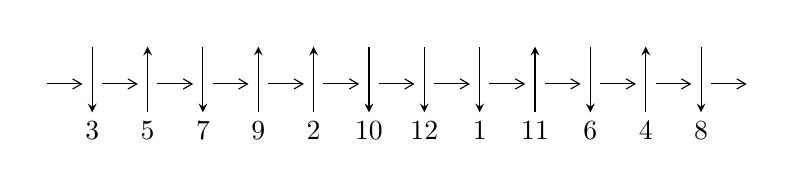
\begin{tikzpicture}[x=20pt, y=17pt]
	% nodes
	\node (C0) at (0, 0) {};
	\node (C1) at (1, 0) {};
	\node (C1U) at (1, +1) {};
	\node (C1D) at (1, -1) {3};

	\node (C2) at (2, 0) {};
	\node (C2U) at (2, +1) {};
	\node (C2D) at (2, -1) {5};

	\node (C3) at (3, 0) {};
	\node (C3U) at (3, +1) {};
	\node (C3D) at (3, -1) {7};

	\node (C4) at (4, 0) {};
	\node (C4U) at (4, +1) {};
	\node (C4D) at (4, -1) {9};

	\node (C5) at (5, 0) {};
	\node (C5U) at (5, +1) {};
	\node (C5D) at (5, -1) {2};

	\node (C6) at (6, 0) {};
	\node (C6U) at (6, +1) {};
	\node (C6D) at (6, -1) {10};

	\node (C7) at (7, 0) {};
	\node (C7U) at (7, +1) {};
	\node (C7D) at (7, -1) {12};

	\node (C8) at (8, 0) {};
	\node (C8U) at (8, +1) {};
	\node (C8D) at (8, -1) {1};

	\node (C9) at (9, 0) {};
	\node (C9U) at (9, +1) {};
	\node (C9D) at (9, -1) {11};

	\node (C10) at (10, 0) {};
	\node (C10U) at (10, +1) {};
	\node (C10D) at (10, -1) {6};

	\node (C11) at (11, 0) {};
	\node (C11U) at (11, +1) {};
	\node (C11D) at (11, -1) {4};

	\node (C12) at (12, 0) {};
	\node (C12U) at (12, +1) {};
	\node (C12D) at (12, -1) {8};
	\node (C13) at (13, 0) {};

	% arrows
	\draw[->,>={angle 60}]
	(C0) edge (C1) (C1) edge (C2) (C2) edge (C3) (C3) edge (C4) (C4) edge (C5) (C5) edge (C6) (C6) edge (C7) (C7) edge (C8) (C8) edge (C9) (C9) edge (C10) (C10) edge (C11) (C11) edge (C12) (C12) edge (C13) ;	\draw[->,>=stealth]
	(C1U) edge (C1D) (C2D) edge (C2U) (C3U) edge (C3D) (C4D) edge (C4U) (C5D) edge (C5U) (C6U) edge (C6D) (C7U) edge (C7D) (C8U) edge (C8D) (C9D) edge (C9U) (C10U) edge (C10D) (C11D) edge (C11U) (C12U) edge (C12D) ;
	\end{tikzpicture} \\
\hhline{~~} \\& 
\textbf{Solving Sequence} \\ \cline{2-2} 
 &
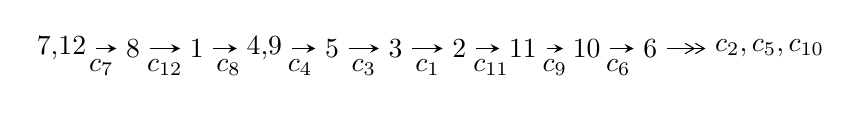
\begin{tikzpicture}[x=23pt, y=7pt]
	% node
	\node (A0) at (-1/8, 0) {7,12};
	\node (A1) at (1, 0) {8};
	\node (A2) at (2, 0) {1};
	\node (A3) at (49/16, 0) {4,9};
	\node (A4) at (33/8, 0) {5};
	\node (A5) at (41/8, 0) {3};
	\node (A6) at (49/8, 0) {2};
	\node (A7) at (57/8, 0) {11};
	\node (A8) at (65/8, 0) {10};
	\node (A9) at (73/8, 0) {6};
	\node (C1) at (1/2, -1) {$c_{7}$};
	\node (C2) at (3/2, -1) {$c_{12}$};
	\node (C3) at (5/2, -1) {$c_{8}$};
	\node (C4) at (29/8, -1) {$c_{4}$};
	\node (C5) at (37/8, -1) {$c_{3}$};
	\node (C6) at (45/8, -1) {$c_{1}$};
	\node (C7) at (53/8, -1) {$c_{11}$};
	\node (C8) at (61/8, -1) {$c_{9}$};
	\node (C9) at (69/8, -1) {$c_{6}$};
	\node (A10) at (11, 0) {$c_{2},c_{5},c_{10}$};

	% edge
	\draw[->,>=stealth]	
	(A0) edge (A1) (A1) edge (A2) (A2) edge (A3) (A3) edge (A4) (A4) edge (A5) (A5) edge (A6) (A6) edge (A7) (A7) edge (A8) (A8) edge (A9) ;
	\draw[->>,>={angle 60}]	
	(A9) edge (A10);
\end{tikzpicture} \\ 

\end{tabular} \\

\footnotetext{
The image of knot diagram is generated by the software ``\textbf{Draw programme}" developed by Andrew Bartholomew(\url{http://www.layer8.co.uk/maths/draw/index.htm\#Running-draw}), where we modified some parts for our purpose(\url{https://github.com/CATsTAILs/LinksPainter}).
}\phantom \\ \newline 
\centering \textbf{Ideals for irreducible components\footnotemark of $X_{\text{par}}$} 
 
\begin{align*}
I^u_{1}&=\langle 
9.06148\times10^{225} u^{108}+1.05422\times10^{226} u^{107}+\cdots+5.27836\times10^{225} b+1.18579\times10^{226},\\
\phantom{I^u_{1}}&\phantom{= \langle  }-3.01470\times10^{223} u^{108}-3.51077\times10^{223} u^{107}+\cdots+5.38608\times10^{223} a-7.22964\times10^{223},\\
\phantom{I^u_{1}}&\phantom{= \langle  }u^{109}+3 u^{108}+\cdots+2 u^2+1\rangle \\
I^u_{2}&=\langle 
21 u^2 b+49 b^2+35 b u+10 u^2+7 b+19 u+22,\;a,\;u^3+u^2-1\rangle \\
\\
\end{align*}
\raggedright * 2 irreducible components of $\dim_{\mathbb{C}}=0$, with total 115 representations.\\
\footnotetext{All coefficients of polynomials are rational numbers. But the coefficients are sometimes approximated in decimal forms when there is not enough margin.}
\newpage
\renewcommand{\arraystretch}{1}
\centering \section*{I. $I^u_{1}= \langle 9.06\times10^{225} u^{108}+1.05\times10^{226} u^{107}+\cdots+5.28\times10^{225} b+1.19\times10^{226},\;-3.01\times10^{223} u^{108}-3.51\times10^{223} u^{107}+\cdots+5.39\times10^{223} a-7.23\times10^{223},\;u^{109}+3 u^{108}+\cdots+2 u^2+1 \rangle$}
\flushleft \textbf{(i) Arc colorings}\\
\begin{tabular}{m{7pt} m{180pt} m{7pt} m{180pt} }
\flushright $a_{7}=$&$\begin{pmatrix}1\\0\end{pmatrix}$ \\
\flushright $a_{12}=$&$\begin{pmatrix}0\\u\end{pmatrix}$ \\
\flushright $a_{8}=$&$\begin{pmatrix}1\\u^2\end{pmatrix}$ \\
\flushright $a_{1}=$&$\begin{pmatrix}- u\\- u^3+u\end{pmatrix}$ \\
\flushright $a_{4}=$&$\begin{pmatrix}0.559721 u^{108}+0.651823 u^{107}+\cdots-0.410187 u+1.34228\\-1.71672 u^{108}-1.99725 u^{107}+\cdots+3.05241 u-2.24651\end{pmatrix}$ \\
\flushright $a_{9}=$&$\begin{pmatrix}- u^2+1\\- u^4+2 u^2\end{pmatrix}$ \\
\flushright $a_{5}=$&$\begin{pmatrix}0.192858 u^{108}+0.779830 u^{107}+\cdots+2.58086 u+0.364839\\-0.692306 u^{108}-0.275910 u^{107}+\cdots+1.29823 u-1.50459\end{pmatrix}$ \\
\flushright $a_{3}=$&$\begin{pmatrix}-1.15700 u^{108}-1.34542 u^{107}+\cdots+2.64222 u-0.904224\\-1.71672 u^{108}-1.99725 u^{107}+\cdots+3.05241 u-2.24651\end{pmatrix}$ \\
\flushright $a_{2}=$&$\begin{pmatrix}-4.03867 u^{108}-6.47872 u^{107}+\cdots+0.850657 u-3.08463\\-3.85538 u^{108}-6.16675 u^{107}+\cdots+6.51846 u-3.48949\end{pmatrix}$ \\
\flushright $a_{11}=$&$\begin{pmatrix}0.107568 u^{108}+0.213955 u^{107}+\cdots+0.809172 u-0.177700\\1.39394 u^{108}+2.20200 u^{107}+\cdots-1.98924 u+1.33556\end{pmatrix}$ \\
\flushright $a_{10}=$&$\begin{pmatrix}-0.222413 u^{108}-0.429613 u^{107}+\cdots-0.690353 u+0.836754\\1.26981 u^{108}+2.30353 u^{107}+\cdots+0.348221 u+1.14552\end{pmatrix}$ \\
\flushright $a_{6}=$&$\begin{pmatrix}-1.03789 u^{108}-1.77503 u^{107}+\cdots+1.07250 u-1.04911\\-0.967747 u^{108}-1.68509 u^{107}+\cdots-0.843787 u-0.111823\end{pmatrix}$\\&\end{tabular}
\flushleft \textbf{(ii) Obstruction class $= -1$}\\~\\
\flushleft \textbf{(iii) Cusp Shapes $= 10.5657 u^{108}+18.1769 u^{107}+\cdots+8.33675 u+11.3613$}\\~\\
\newpage\renewcommand{\arraystretch}{1}
\flushleft \textbf{(iv) u-Polynomials at the component}\newline \\
\begin{tabular}{m{50pt}|m{274pt}}
Crossings & \hspace{64pt}u-Polynomials at each crossing \\
\hline $$\begin{aligned}c_{1}\end{aligned}$$&$\begin{aligned}
&u^{109}+50 u^{108}+\cdots-9999 u-2401
\end{aligned}$\\
\hline $$\begin{aligned}c_{2},c_{5}\end{aligned}$$&$\begin{aligned}
&u^{109}+4 u^{108}+\cdots-551 u-49
\end{aligned}$\\
\hline $$\begin{aligned}c_{3}\end{aligned}$$&$\begin{aligned}
&49(49 u^{109}+42 u^{108}+\cdots-1346644 u-153031)
\end{aligned}$\\
\hline $$\begin{aligned}c_{4}\end{aligned}$$&$\begin{aligned}
&49(49 u^{109}+154 u^{108}+\cdots+1.84924\times10^{7} u+1398784)
\end{aligned}$\\
\hline $$\begin{aligned}c_{6},c_{10}\end{aligned}$$&$\begin{aligned}
&u^{109}+3 u^{108}+\cdots+6 u+1
\end{aligned}$\\
\hline $$\begin{aligned}c_{7},c_{8},c_{12}\end{aligned}$$&$\begin{aligned}
&u^{109}+3 u^{108}+\cdots+2 u^2+1
\end{aligned}$\\
\hline $$\begin{aligned}c_{9}\end{aligned}$$&$\begin{aligned}
&u^{109}-49 u^{108}+\cdots-4 u+1
\end{aligned}$\\
\hline $$\begin{aligned}c_{11}\end{aligned}$$&$\begin{aligned}
&u^{109}-5 u^{108}+\cdots+48608 u+21952
\end{aligned}$\\
\hline
\end{tabular}\\~\\
\newpage\renewcommand{\arraystretch}{1}
\flushleft \textbf{(v) Riley Polynomials at the component}\newline \\
\begin{tabular}{m{50pt}|m{274pt}}
Crossings & \hspace{64pt}Riley Polynomials at each crossing \\
\hline $$\begin{aligned}c_{1}\end{aligned}$$&$\begin{aligned}
&y^{109}+22 y^{108}+\cdots+18653329 y-5764801
\end{aligned}$\\
\hline $$\begin{aligned}c_{2},c_{5}\end{aligned}$$&$\begin{aligned}
&y^{109}+50 y^{108}+\cdots-9999 y-2401
\end{aligned}$\\
\hline $$\begin{aligned}c_{3}\end{aligned}$$&$\begin{aligned}
&2401\\
&\cdot(2401 y^{109}-163660 y^{108}+\cdots-913616530238 y-23418486961)
\end{aligned}$\\
\hline $$\begin{aligned}c_{4}\end{aligned}$$&$\begin{aligned}
&2401\\
&\cdot(2401 y^{109}+1666 y^{108}+\cdots+9951035523072 y-1956596678656)
\end{aligned}$\\
\hline $$\begin{aligned}c_{6},c_{10}\end{aligned}$$&$\begin{aligned}
&y^{109}+49 y^{108}+\cdots-4 y-1
\end{aligned}$\\
\hline $$\begin{aligned}c_{7},c_{8},c_{12}\end{aligned}$$&$\begin{aligned}
&y^{109}-103 y^{108}+\cdots-4 y-1
\end{aligned}$\\
\hline $$\begin{aligned}c_{9}\end{aligned}$$&$\begin{aligned}
&y^{109}+25 y^{108}+\cdots+72 y-1
\end{aligned}$\\
\hline $$\begin{aligned}c_{11}\end{aligned}$$&$\begin{aligned}
&y^{109}+35 y^{108}+\cdots-3911670784 y-481890304
\end{aligned}$\\
\hline
\end{tabular}\\~\\
\newpage\flushleft \textbf{(vi) Complex Volumes and Cusp Shapes}
$$\begin{array}{c|c|c}  
\text{Solutions to }I^u_{1}& \I (\text{vol} + \sqrt{-1}CS) & \text{Cusp shape}\\
 \hline 
\begin{aligned}
u &= -0.489926 + 0.841164 I \\
a &= -0.606125 + 1.170680 I \\
b &= \phantom{-}1.134530 - 0.822129 I\end{aligned}
 & -2.69398 + 8.51191 I & \phantom{-0.000000 } 0 \\ \hline\begin{aligned}
u &= -0.489926 - 0.841164 I \\
a &= -0.606125 - 1.170680 I \\
b &= \phantom{-}1.134530 + 0.822129 I\end{aligned}
 & -2.69398 - 8.51191 I & \phantom{-0.000000 } 0 \\ \hline\begin{aligned}
u &= \phantom{-}0.509943 + 0.826525 I \\
a &= \phantom{-}0.50185 + 1.38603 I \\
b &= -1.12948 - 1.03666 I\end{aligned}
 & -0.5579 - 14.3486 I & \phantom{-0.000000 } 0 \\ \hline\begin{aligned}
u &= \phantom{-}0.509943 - 0.826525 I \\
a &= \phantom{-}0.50185 - 1.38603 I \\
b &= -1.12948 + 1.03666 I\end{aligned}
 & -0.5579 + 14.3486 I & \phantom{-0.000000 } 0 \\ \hline\begin{aligned}
u &= \phantom{-}0.648459 + 0.806149 I \\
a &= \phantom{-}1.065950 + 0.105647 I \\
b &= -0.773273 + 0.689039 I\end{aligned}
 & -0.92733 + 8.91163 I & \phantom{-0.000000 } 0 \\ \hline\begin{aligned}
u &= \phantom{-}0.648459 - 0.806149 I \\
a &= \phantom{-}1.065950 - 0.105647 I \\
b &= -0.773273 - 0.689039 I\end{aligned}
 & -0.92733 - 8.91163 I & \phantom{-0.000000 } 0 \\ \hline\begin{aligned}
u &= -0.705187 + 0.776451 I \\
a &= -0.857316 + 0.368561 I \\
b &= \phantom{-}0.796547 + 0.451101 I\end{aligned}
 & -3.29024 - 3.05508 I & \phantom{-0.000000 } 0 \\ \hline\begin{aligned}
u &= -0.705187 - 0.776451 I \\
a &= -0.857316 - 0.368561 I \\
b &= \phantom{-}0.796547 - 0.451101 I\end{aligned}
 & -3.29024 + 3.05508 I & \phantom{-0.000000 } 0 \\ \hline\begin{aligned}
u &= \phantom{-}0.520207 + 0.931345 I \\
a &= \phantom{-}0.253538 + 0.739970 I \\
b &= -0.677677 - 0.603783 I\end{aligned}
 & \phantom{-}3.72190 - 5.56725 I & \phantom{-0.000000 } 0 \\ \hline\begin{aligned}
u &= \phantom{-}0.520207 - 0.931345 I \\
a &= \phantom{-}0.253538 - 0.739970 I \\
b &= -0.677677 + 0.603783 I\end{aligned}
 & \phantom{-}3.72190 + 5.56725 I & \phantom{-0.000000 } 0\\
 \hline 
 \end{array}$$\newpage$$\begin{array}{c|c|c}  
\text{Solutions to }I^u_{1}& \I (\text{vol} + \sqrt{-1}CS) & \text{Cusp shape}\\
 \hline 
\begin{aligned}
u &= -0.332705 + 0.846613 I \\
a &= -0.994225 + 0.334332 I \\
b &= \phantom{-}1.147690 + 0.019200 I\end{aligned}
 & -4.05789 + 3.74836 I & \phantom{-0.000000 } 0 \\ \hline\begin{aligned}
u &= -0.332705 - 0.846613 I \\
a &= -0.994225 - 0.334332 I \\
b &= \phantom{-}1.147690 - 0.019200 I\end{aligned}
 & -4.05789 - 3.74836 I & \phantom{-0.000000 } 0 \\ \hline\begin{aligned}
u &= \phantom{-}0.362269 + 0.817846 I \\
a &= -0.241246 - 1.015470 I \\
b &= \phantom{-}0.522740 + 0.796545 I\end{aligned}
 & \phantom{-}4.88494 - 0.80424 I & \phantom{-0.000000 } 0 \\ \hline\begin{aligned}
u &= \phantom{-}0.362269 - 0.817846 I \\
a &= -0.241246 + 1.015470 I \\
b &= \phantom{-}0.522740 - 0.796545 I\end{aligned}
 & \phantom{-}4.88494 + 0.80424 I & \phantom{-0.000000 } 0 \\ \hline\begin{aligned}
u &= \phantom{-}0.640718 + 0.619636 I \\
a &= -1.130640 - 0.166942 I \\
b &= \phantom{-}0.673295 - 0.437255 I\end{aligned}
 & \phantom{-}0.92415 + 4.09684 I & \phantom{-0.000000 } 0 \\ \hline\begin{aligned}
u &= \phantom{-}0.640718 - 0.619636 I \\
a &= -1.130640 + 0.166942 I \\
b &= \phantom{-}0.673295 + 0.437255 I\end{aligned}
 & \phantom{-}0.92415 - 4.09684 I & \phantom{-0.000000 } 0 \\ \hline\begin{aligned}
u &= -0.821915 + 0.342724 I \\
a &= \phantom{-}0.666369 - 0.371402 I \\
b &= -0.172804 - 0.223629 I\end{aligned}
 & -1.34681 + 0.71674 I & \phantom{-0.000000 } 0 \\ \hline\begin{aligned}
u &= -0.821915 - 0.342724 I \\
a &= \phantom{-}0.666369 + 0.371402 I \\
b &= -0.172804 + 0.223629 I\end{aligned}
 & -1.34681 - 0.71674 I & \phantom{-0.000000 } 0 \\ \hline\begin{aligned}
u &= \phantom{-}0.438488 + 0.747759 I \\
a &= -0.60734 - 1.53057 I \\
b &= \phantom{-}0.973424 + 0.926486 I\end{aligned}
 & \phantom{-}1.56612 - 8.78514 I & \phantom{-0.000000 } 0 \\ \hline\begin{aligned}
u &= \phantom{-}0.438488 - 0.747759 I \\
a &= -0.60734 + 1.53057 I \\
b &= \phantom{-}0.973424 - 0.926486 I\end{aligned}
 & \phantom{-}1.56612 + 8.78514 I & \phantom{-0.000000 } 0\\
 \hline 
 \end{array}$$\newpage$$\begin{array}{c|c|c}  
\text{Solutions to }I^u_{1}& \I (\text{vol} + \sqrt{-1}CS) & \text{Cusp shape}\\
 \hline 
\begin{aligned}
u &= -0.651090 + 0.533274 I \\
a &= -0.28816 + 1.45770 I \\
b &= \phantom{-}1.062210 - 0.259698 I\end{aligned}
 & -5.38646 + 0.84334 I & \phantom{-0.000000 } 0 \\ \hline\begin{aligned}
u &= -0.651090 - 0.533274 I \\
a &= -0.28816 - 1.45770 I \\
b &= \phantom{-}1.062210 + 0.259698 I\end{aligned}
 & -5.38646 - 0.84334 I & \phantom{-0.000000 } 0 \\ \hline\begin{aligned}
u &= -0.416063 + 0.725434 I \\
a &= \phantom{-}0.68573 - 1.28827 I \\
b &= -0.903118 + 0.735994 I\end{aligned}
 & -0.49874 + 3.40197 I & \phantom{-0.000000 } 0 \\ \hline\begin{aligned}
u &= -0.416063 - 0.725434 I \\
a &= \phantom{-}0.68573 + 1.28827 I \\
b &= -0.903118 - 0.735994 I\end{aligned}
 & -0.49874 - 3.40197 I & \phantom{-0.000000 } 0 \\ \hline\begin{aligned}
u &= \phantom{-}0.251562 + 0.774587 I \\
a &= \phantom{-}1.165860 - 0.068813 I \\
b &= -1.137790 + 0.418799 I\end{aligned}
 & -3.07379 + 2.21369 I & \phantom{-0.000000 } 0 \\ \hline\begin{aligned}
u &= \phantom{-}0.251562 - 0.774587 I \\
a &= \phantom{-}1.165860 + 0.068813 I \\
b &= -1.137790 - 0.418799 I\end{aligned}
 & -3.07379 - 2.21369 I & \phantom{-0.000000 } 0 \\ \hline\begin{aligned}
u &= \phantom{-}0.579115 + 0.507577 I \\
a &= \phantom{-}0.05747 + 1.87013 I \\
b &= -1.137540 - 0.504304 I\end{aligned}
 & -4.32288 - 6.26751 I & \phantom{-0.000000 } 0 \\ \hline\begin{aligned}
u &= \phantom{-}0.579115 - 0.507577 I \\
a &= \phantom{-}0.05747 - 1.87013 I \\
b &= -1.137540 + 0.504304 I\end{aligned}
 & -4.32288 + 6.26751 I & \phantom{-0.000000 } 0 \\ \hline\begin{aligned}
u &= \phantom{-}1.013290 + 0.706462 I \\
a &= -0.425669 - 0.055355 I \\
b &= \phantom{-}0.197913 - 0.411645 I\end{aligned}
 & \phantom{-}3.19213 - 4.51638 I & \phantom{-0.000000 } 0 \\ \hline\begin{aligned}
u &= \phantom{-}1.013290 - 0.706462 I \\
a &= -0.425669 + 0.055355 I \\
b &= \phantom{-}0.197913 + 0.411645 I\end{aligned}
 & \phantom{-}3.19213 + 4.51638 I & \phantom{-0.000000 } 0\\
 \hline 
 \end{array}$$\newpage$$\begin{array}{c|c|c}  
\text{Solutions to }I^u_{1}& \I (\text{vol} + \sqrt{-1}CS) & \text{Cusp shape}\\
 \hline 
\begin{aligned}
u &= \phantom{-}0.935705 + 0.861076 I \\
a &= \phantom{-}0.293724 + 0.261994 I \\
b &= -0.468609 + 0.170672 I\end{aligned}
 & \phantom{-}2.71396 - 0.69644 I & \phantom{-0.000000 } 0 \\ \hline\begin{aligned}
u &= \phantom{-}0.935705 - 0.861076 I \\
a &= \phantom{-}0.293724 - 0.261994 I \\
b &= -0.468609 - 0.170672 I\end{aligned}
 & \phantom{-}2.71396 + 0.69644 I & \phantom{-0.000000 } 0 \\ \hline\begin{aligned}
u &= \phantom{-}1.280350 + 0.018606 I \\
a &= -1.43758 + 0.46050 I \\
b &= -0.179102 - 0.349982 I\end{aligned}
 & -0.30029 - 3.05301 I & \phantom{-0.000000 } 0 \\ \hline\begin{aligned}
u &= \phantom{-}1.280350 - 0.018606 I \\
a &= -1.43758 - 0.46050 I \\
b &= -0.179102 + 0.349982 I\end{aligned}
 & -0.30029 + 3.05301 I & \phantom{-0.000000 } 0 \\ \hline\begin{aligned}
u &= -1.30388\phantom{ +0.000000I} \\
a &= \phantom{-}0.888977\phantom{ +0.000000I} \\
b &= \phantom{-}0.696510\phantom{ +0.000000I}\end{aligned}
 & -2.58592\phantom{ +0.000000I} & \phantom{-0.000000 } 0 \\ \hline\begin{aligned}
u &= -1.303700 + 0.057096 I \\
a &= \phantom{-}0.74284 + 1.24535 I \\
b &= \phantom{-}0.334669 - 0.980720 I\end{aligned}
 & -0.740344 + 0.546849 I & \phantom{-0.000000 } 0 \\ \hline\begin{aligned}
u &= -1.303700 - 0.057096 I \\
a &= \phantom{-}0.74284 - 1.24535 I \\
b &= \phantom{-}0.334669 + 0.980720 I\end{aligned}
 & -0.740344 - 0.546849 I & \phantom{-0.000000 } 0 \\ \hline\begin{aligned}
u &= -0.493875 + 0.488188 I \\
a &= \phantom{-}0.884027 - 0.566340 I \\
b &= -0.585707 + 0.067307 I\end{aligned}
 & -1.18169 + 0.83074 I & -5.14593 - 2.98967 I \\ \hline\begin{aligned}
u &= -0.493875 - 0.488188 I \\
a &= \phantom{-}0.884027 + 0.566340 I \\
b &= -0.585707 - 0.067307 I\end{aligned}
 & -1.18169 - 0.83074 I & -5.14593 + 2.98967 I \\ \hline\begin{aligned}
u &= -1.322990 + 0.037419 I \\
a &= \phantom{-}0.419364 - 0.288008 I \\
b &= \phantom{-}2.24257 - 0.59888 I\end{aligned}
 & -5.13718 + 0.93066 I & \phantom{-0.000000 } 0\\
 \hline 
 \end{array}$$\newpage$$\begin{array}{c|c|c}  
\text{Solutions to }I^u_{1}& \I (\text{vol} + \sqrt{-1}CS) & \text{Cusp shape}\\
 \hline 
\begin{aligned}
u &= -1.322990 - 0.037419 I \\
a &= \phantom{-}0.419364 + 0.288008 I \\
b &= \phantom{-}2.24257 + 0.59888 I\end{aligned}
 & -5.13718 - 0.93066 I & \phantom{-0.000000 } 0 \\ \hline\begin{aligned}
u &= -1.327760 + 0.089354 I \\
a &= -0.08728 + 1.59023 I \\
b &= \phantom{-}0.294552 - 1.028630 I\end{aligned}
 & -1.54532 + 6.50144 I & \phantom{-0.000000 } 0 \\ \hline\begin{aligned}
u &= -1.327760 - 0.089354 I \\
a &= -0.08728 - 1.59023 I \\
b &= \phantom{-}0.294552 + 1.028630 I\end{aligned}
 & -1.54532 - 6.50144 I & \phantom{-0.000000 } 0 \\ \hline\begin{aligned}
u &= \phantom{-}1.346210 + 0.060339 I \\
a &= -0.006328 + 0.929324 I \\
b &= -0.225605 - 1.369110 I\end{aligned}
 & -3.32385 - 2.89150 I & \phantom{-0.000000 } 0 \\ \hline\begin{aligned}
u &= \phantom{-}1.346210 - 0.060339 I \\
a &= -0.006328 - 0.929324 I \\
b &= -0.225605 + 1.369110 I\end{aligned}
 & -3.32385 + 2.89150 I & \phantom{-0.000000 } 0 \\ \hline\begin{aligned}
u &= \phantom{-}1.364470 + 0.020474 I \\
a &= -0.295490 - 0.214355 I \\
b &= -4.33439 + 0.52295 I\end{aligned}
 & -4.95461 + 3.75362 I & \phantom{-0.000000 } 0 \\ \hline\begin{aligned}
u &= \phantom{-}1.364470 - 0.020474 I \\
a &= -0.295490 + 0.214355 I \\
b &= -4.33439 - 0.52295 I\end{aligned}
 & -4.95461 - 3.75362 I & \phantom{-0.000000 } 0 \\ \hline\begin{aligned}
u &= \phantom{-}1.373840 + 0.099861 I \\
a &= \phantom{-}0.819714 + 0.934876 I \\
b &= \phantom{-}0.250264 - 0.590954 I\end{aligned}
 & -2.88115 - 3.30978 I & \phantom{-0.000000 } 0 \\ \hline\begin{aligned}
u &= \phantom{-}1.373840 - 0.099861 I \\
a &= \phantom{-}0.819714 - 0.934876 I \\
b &= \phantom{-}0.250264 + 0.590954 I\end{aligned}
 & -2.88115 + 3.30978 I & \phantom{-0.000000 } 0 \\ \hline\begin{aligned}
u &= \phantom{-}1.405360 + 0.131951 I \\
a &= \phantom{-}1.51446 + 0.37423 I \\
b &= \phantom{-}0.346042 + 0.380484 I\end{aligned}
 & -4.85566 - 8.88179 I & \phantom{-0.000000 } 0\\
 \hline 
 \end{array}$$\newpage$$\begin{array}{c|c|c}  
\text{Solutions to }I^u_{1}& \I (\text{vol} + \sqrt{-1}CS) & \text{Cusp shape}\\
 \hline 
\begin{aligned}
u &= \phantom{-}1.405360 - 0.131951 I \\
a &= \phantom{-}1.51446 - 0.37423 I \\
b &= \phantom{-}0.346042 - 0.380484 I\end{aligned}
 & -4.85566 + 8.88179 I & \phantom{-0.000000 } 0 \\ \hline\begin{aligned}
u &= -1.42243 + 0.11797 I \\
a &= -1.192690 + 0.117412 I \\
b &= -0.762736 + 0.416056 I\end{aligned}
 & -6.25207 + 4.41292 I & \phantom{-0.000000 } 0 \\ \hline\begin{aligned}
u &= -1.42243 - 0.11797 I \\
a &= -1.192690 - 0.117412 I \\
b &= -0.762736 - 0.416056 I\end{aligned}
 & -6.25207 - 4.41292 I & \phantom{-0.000000 } 0 \\ \hline\begin{aligned}
u &= \phantom{-}1.44211 + 0.02977 I \\
a &= \phantom{-}0.303260 - 0.075434 I \\
b &= \phantom{-}4.14471 + 2.85875 I\end{aligned}
 & -5.17776 + 0.09499 I & \phantom{-0.000000 } 0 \\ \hline\begin{aligned}
u &= \phantom{-}1.44211 - 0.02977 I \\
a &= \phantom{-}0.303260 + 0.075434 I \\
b &= \phantom{-}4.14471 - 2.85875 I\end{aligned}
 & -5.17776 - 0.09499 I & \phantom{-0.000000 } 0 \\ \hline\begin{aligned}
u &= -1.44737 + 0.07794 I \\
a &= -0.658075 - 0.070611 I \\
b &= -1.61466 + 0.78393 I\end{aligned}
 & -6.17975 + 3.74343 I & \phantom{-0.000000 } 0 \\ \hline\begin{aligned}
u &= -1.44737 - 0.07794 I \\
a &= -0.658075 + 0.070611 I \\
b &= -1.61466 - 0.78393 I\end{aligned}
 & -6.17975 - 3.74343 I & \phantom{-0.000000 } 0 \\ \hline\begin{aligned}
u &= -1.45325 + 0.17426 I \\
a &= -0.022009 + 0.560798 I \\
b &= \phantom{-}1.191190 - 0.354754 I\end{aligned}
 & -5.88811 - 1.65848 I & \phantom{-0.000000 } 0 \\ \hline\begin{aligned}
u &= -1.45325 - 0.17426 I \\
a &= -0.022009 - 0.560798 I \\
b &= \phantom{-}1.191190 + 0.354754 I\end{aligned}
 & -5.88811 + 1.65848 I & \phantom{-0.000000 } 0 \\ \hline\begin{aligned}
u &= \phantom{-}1.46074 + 0.22397 I \\
a &= -0.087044 + 0.735866 I \\
b &= -1.246400 - 0.536367 I\end{aligned}
 & -7.30379 - 3.60572 I & \phantom{-0.000000 } 0\\
 \hline 
 \end{array}$$\newpage$$\begin{array}{c|c|c}  
\text{Solutions to }I^u_{1}& \I (\text{vol} + \sqrt{-1}CS) & \text{Cusp shape}\\
 \hline 
\begin{aligned}
u &= \phantom{-}1.46074 - 0.22397 I \\
a &= -0.087044 - 0.735866 I \\
b &= -1.246400 + 0.536367 I\end{aligned}
 & -7.30379 + 3.60572 I & \phantom{-0.000000 } 0 \\ \hline\begin{aligned}
u &= \phantom{-}0.517939 + 0.030277 I \\
a &= -1.257170 - 0.613936 I \\
b &= \phantom{-}0.585738 + 0.551331 I\end{aligned}
 & \phantom{-}0.80173 + 2.83553 I & -4.73944 - 4.73337 I \\ \hline\begin{aligned}
u &= \phantom{-}0.517939 - 0.030277 I \\
a &= -1.257170 + 0.613936 I \\
b &= \phantom{-}0.585738 - 0.551331 I\end{aligned}
 & \phantom{-}0.80173 - 2.83553 I & -4.73944 + 4.73337 I \\ \hline\begin{aligned}
u &= -0.268706 + 0.441472 I \\
a &= \phantom{-}2.76472 + 1.19560 I \\
b &= \phantom{-}0.174119 - 0.914672 I\end{aligned}
 & \phantom{-}0.49351 + 6.83165 I & \phantom{-}0.30272 - 12.02369 I \\ \hline\begin{aligned}
u &= -0.268706 - 0.441472 I \\
a &= \phantom{-}2.76472 - 1.19560 I \\
b &= \phantom{-}0.174119 + 0.914672 I\end{aligned}
 & \phantom{-}0.49351 - 6.83165 I & \phantom{-}0.30272 + 12.02369 I \\ \hline\begin{aligned}
u &= -1.46682 + 0.28160 I \\
a &= \phantom{-}0.432061 + 0.746282 I \\
b &= \phantom{-}0.980677 - 0.924511 I\end{aligned}
 & -1.01642 + 4.71566 I & \phantom{-0.000000 } 0 \\ \hline\begin{aligned}
u &= -1.46682 - 0.28160 I \\
a &= \phantom{-}0.432061 - 0.746282 I \\
b &= \phantom{-}0.980677 + 0.924511 I\end{aligned}
 & -1.01642 - 4.71566 I & \phantom{-0.000000 } 0 \\ \hline\begin{aligned}
u &= \phantom{-}0.316309 + 0.384190 I \\
a &= -1.93029 + 1.27801 I \\
b &= -0.506253 - 0.870148 I\end{aligned}
 & -0.67357 - 2.60087 I & -3.21300 + 6.51215 I \\ \hline\begin{aligned}
u &= \phantom{-}0.316309 - 0.384190 I \\
a &= -1.93029 - 1.27801 I \\
b &= -0.506253 + 0.870148 I\end{aligned}
 & -0.67357 + 2.60087 I & -3.21300 - 6.51215 I \\ \hline\begin{aligned}
u &= -1.46418 + 0.35096 I \\
a &= \phantom{-}0.061766 - 0.696071 I \\
b &= -1.204820 - 0.108656 I\end{aligned}
 & -8.55069 + 2.04352 I & \phantom{-0.000000 } 0\\
 \hline 
 \end{array}$$\newpage$$\begin{array}{c|c|c}  
\text{Solutions to }I^u_{1}& \I (\text{vol} + \sqrt{-1}CS) & \text{Cusp shape}\\
 \hline 
\begin{aligned}
u &= -1.46418 - 0.35096 I \\
a &= \phantom{-}0.061766 + 0.696071 I \\
b &= -1.204820 + 0.108656 I\end{aligned}
 & -8.55069 - 2.04352 I & \phantom{-0.000000 } 0 \\ \hline\begin{aligned}
u &= \phantom{-}1.48529 + 0.26251 I \\
a &= -0.349746 + 0.983137 I \\
b &= -1.32341 - 0.99961 I\end{aligned}
 & -6.67106 - 7.00396 I & \phantom{-0.000000 } 0 \\ \hline\begin{aligned}
u &= \phantom{-}1.48529 - 0.26251 I \\
a &= -0.349746 - 0.983137 I \\
b &= -1.32341 + 0.99961 I\end{aligned}
 & -6.67106 + 7.00396 I & \phantom{-0.000000 } 0 \\ \hline\begin{aligned}
u &= \phantom{-}0.027486 + 0.487190 I \\
a &= -0.96250 - 2.69226 I \\
b &= \phantom{-}0.177661 + 0.847878 I\end{aligned}
 & \phantom{-}3.12289 + 1.30549 I & \phantom{-}8.69976 - 1.36522 I \\ \hline\begin{aligned}
u &= \phantom{-}0.027486 - 0.487190 I \\
a &= -0.96250 + 2.69226 I \\
b &= \phantom{-}0.177661 - 0.847878 I\end{aligned}
 & \phantom{-}3.12289 - 1.30549 I & \phantom{-}8.69976 + 1.36522 I \\ \hline\begin{aligned}
u &= -1.49169 + 0.26804 I \\
a &= \phantom{-}0.449384 + 1.049550 I \\
b &= \phantom{-}1.33215 - 1.16283 I\end{aligned}
 & -4.69085 + 12.48030 I & \phantom{-0.000000 } 0 \\ \hline\begin{aligned}
u &= -1.49169 - 0.26804 I \\
a &= \phantom{-}0.449384 - 1.049550 I \\
b &= \phantom{-}1.33215 + 1.16283 I\end{aligned}
 & -4.69085 - 12.48030 I & \phantom{-0.000000 } 0 \\ \hline\begin{aligned}
u &= -1.50759 + 0.17219 I \\
a &= -0.617594 - 1.177080 I \\
b &= -1.17609 + 0.78971 I\end{aligned}
 & -11.1073 + 8.7748 I & \phantom{-0.000000 } 0 \\ \hline\begin{aligned}
u &= -1.50759 - 0.17219 I \\
a &= -0.617594 + 1.177080 I \\
b &= -1.17609 - 0.78971 I\end{aligned}
 & -11.1073 - 8.7748 I & \phantom{-0.000000 } 0 \\ \hline\begin{aligned}
u &= \phantom{-}0.086000 + 0.474332 I \\
a &= -2.43919 - 1.92635 I \\
b &= \phantom{-}0.367378 + 0.456437 I\end{aligned}
 & \phantom{-}2.74605 - 4.56330 I & \phantom{-}6.84455 + 8.54463 I\\
 \hline 
 \end{array}$$\newpage$$\begin{array}{c|c|c}  
\text{Solutions to }I^u_{1}& \I (\text{vol} + \sqrt{-1}CS) & \text{Cusp shape}\\
 \hline 
\begin{aligned}
u &= \phantom{-}0.086000 - 0.474332 I \\
a &= -2.43919 + 1.92635 I \\
b &= \phantom{-}0.367378 - 0.456437 I\end{aligned}
 & \phantom{-}2.74605 + 4.56330 I & \phantom{-}6.84455 - 8.54463 I \\ \hline\begin{aligned}
u &= \phantom{-}1.49415 + 0.33116 I \\
a &= \phantom{-}0.076295 - 0.792286 I \\
b &= \phantom{-}1.375540 + 0.230057 I\end{aligned}
 & -9.99282 - 8.09149 I & \phantom{-0.000000 } 0 \\ \hline\begin{aligned}
u &= \phantom{-}1.49415 - 0.33116 I \\
a &= \phantom{-}0.076295 + 0.792286 I \\
b &= \phantom{-}1.375540 - 0.230057 I\end{aligned}
 & -9.99282 + 8.09149 I & \phantom{-0.000000 } 0 \\ \hline\begin{aligned}
u &= \phantom{-}1.52357 + 0.17118 I \\
a &= \phantom{-}0.421306 - 1.094450 I \\
b &= \phantom{-}1.124160 + 0.649554 I\end{aligned}
 & -12.44990 - 3.40335 I & \phantom{-0.000000 } 0 \\ \hline\begin{aligned}
u &= \phantom{-}1.52357 - 0.17118 I \\
a &= \phantom{-}0.421306 + 1.094450 I \\
b &= \phantom{-}1.124160 - 0.649554 I\end{aligned}
 & -12.44990 + 3.40335 I & \phantom{-0.000000 } 0 \\ \hline\begin{aligned}
u &= -0.160251 + 0.432564 I \\
a &= \phantom{-}2.74408 - 0.38939 I \\
b &= -0.076446 - 0.185049 I\end{aligned}
 & \phantom{-}1.93549 + 1.48976 I & \phantom{-}4.80637 - 4.55092 I \\ \hline\begin{aligned}
u &= -0.160251 - 0.432564 I \\
a &= \phantom{-}2.74408 + 0.38939 I \\
b &= -0.076446 + 0.185049 I\end{aligned}
 & \phantom{-}1.93549 - 1.48976 I & \phantom{-}4.80637 + 4.55092 I \\ \hline\begin{aligned}
u &= -1.54980 + 0.09230 I \\
a &= -0.363553 - 0.522923 I \\
b &= -0.543928 + 0.839192 I\end{aligned}
 & -6.36585 + 3.09614 I & \phantom{-0.000000 } 0 \\ \hline\begin{aligned}
u &= -1.54980 - 0.09230 I \\
a &= -0.363553 + 0.522923 I \\
b &= -0.543928 - 0.839192 I\end{aligned}
 & -6.36585 - 3.09614 I & \phantom{-0.000000 } 0 \\ \hline\begin{aligned}
u &= \phantom{-}1.52512 + 0.30119 I \\
a &= \phantom{-}0.381361 - 0.948118 I \\
b &= \phantom{-}1.52384 + 0.96207 I\end{aligned}
 & -9.2312 - 12.6732 I & \phantom{-0.000000 } 0\\
 \hline 
 \end{array}$$\newpage$$\begin{array}{c|c|c}  
\text{Solutions to }I^u_{1}& \I (\text{vol} + \sqrt{-1}CS) & \text{Cusp shape}\\
 \hline 
\begin{aligned}
u &= \phantom{-}1.52512 - 0.30119 I \\
a &= \phantom{-}0.381361 + 0.948118 I \\
b &= \phantom{-}1.52384 - 0.96207 I\end{aligned}
 & -9.2312 + 12.6732 I & \phantom{-0.000000 } 0 \\ \hline\begin{aligned}
u &= -1.53021 + 0.29511 I \\
a &= -0.473162 - 0.979653 I \\
b &= -1.52026 + 1.16960 I\end{aligned}
 & -7.1817 + 18.4464 I & \phantom{-0.000000 } 0 \\ \hline\begin{aligned}
u &= -1.53021 - 0.29511 I \\
a &= -0.473162 + 0.979653 I \\
b &= -1.52026 - 1.16960 I\end{aligned}
 & -7.1817 - 18.4464 I & \phantom{-0.000000 } 0 \\ \hline\begin{aligned}
u &= -0.028029 + 0.432349 I \\
a &= \phantom{-}1.28487 - 1.33272 I \\
b &= -0.012099 + 0.713001 I\end{aligned}
 & \phantom{-}0.85731 + 1.39747 I & \phantom{-}1.09021 - 4.04698 I \\ \hline\begin{aligned}
u &= -0.028029 - 0.432349 I \\
a &= \phantom{-}1.28487 + 1.33272 I \\
b &= -0.012099 - 0.713001 I\end{aligned}
 & \phantom{-}0.85731 - 1.39747 I & \phantom{-}1.09021 + 4.04698 I \\ \hline\begin{aligned}
u &= -1.53867 + 0.32025 I \\
a &= -0.373328 - 0.730198 I \\
b &= -1.096350 + 0.805215 I\end{aligned}
 & -2.93916 + 10.06180 I & \phantom{-0.000000 } 0 \\ \hline\begin{aligned}
u &= -1.53867 - 0.32025 I \\
a &= -0.373328 + 0.730198 I \\
b &= -1.096350 - 0.805215 I\end{aligned}
 & -2.93916 - 10.06180 I & \phantom{-0.000000 } 0 \\ \hline\begin{aligned}
u &= -0.404504 + 0.057065 I \\
a &= \phantom{-}0.83922 - 1.30855 I \\
b &= -0.19631 + 1.74420 I\end{aligned}
 & \phantom{-}0.671600 + 0.217161 I & -12.32084 + 0.43118 I \\ \hline\begin{aligned}
u &= -0.404504 - 0.057065 I \\
a &= \phantom{-}0.83922 + 1.30855 I \\
b &= -0.19631 - 1.74420 I\end{aligned}
 & \phantom{-}0.671600 - 0.217161 I & -12.32084 - 0.43118 I \\ \hline\begin{aligned}
u &= \phantom{-}1.58565 + 0.17300 I \\
a &= \phantom{-}0.029475 - 0.750207 I \\
b &= \phantom{-}0.775362 + 0.263203 I\end{aligned}
 & -11.13310 - 0.27637 I & \phantom{-0.000000 } 0\\
 \hline 
 \end{array}$$\newpage$$\begin{array}{c|c|c}  
\text{Solutions to }I^u_{1}& \I (\text{vol} + \sqrt{-1}CS) & \text{Cusp shape}\\
 \hline 
\begin{aligned}
u &= \phantom{-}1.58565 - 0.17300 I \\
a &= \phantom{-}0.029475 + 0.750207 I \\
b &= \phantom{-}0.775362 - 0.263203 I\end{aligned}
 & -11.13310 + 0.27637 I & \phantom{-0.000000 } 0 \\ \hline\begin{aligned}
u &= \phantom{-}0.317229 + 0.245819 I \\
a &= -1.24995 + 0.85292 I \\
b &= -0.738382 - 0.858373 I\end{aligned}
 & -0.37551 - 2.54693 I & \phantom{-}1.38986 + 6.91010 I \\ \hline\begin{aligned}
u &= \phantom{-}0.317229 - 0.245819 I \\
a &= -1.24995 - 0.85292 I \\
b &= -0.738382 + 0.858373 I\end{aligned}
 & -0.37551 + 2.54693 I & \phantom{-}1.38986 - 6.91010 I \\ \hline\begin{aligned}
u &= \phantom{-}0.214125 + 0.331266 I \\
a &= \phantom{-}0.79698 - 1.33459 I \\
b &= -0.08689 + 2.01105 I\end{aligned}
 & -0.555437 + 0.437836 I & \phantom{-}4.35743 + 8.19634 I \\ \hline\begin{aligned}
u &= \phantom{-}0.214125 - 0.331266 I \\
a &= \phantom{-}0.79698 + 1.33459 I \\
b &= -0.08689 - 2.01105 I\end{aligned}
 & -0.555437 - 0.437836 I & \phantom{-}4.35743 - 8.19634 I \\ \hline\begin{aligned}
u &= -0.295460 + 0.242991 I \\
a &= -0.28861 - 1.62323 I \\
b &= -0.03817 + 2.38617 I\end{aligned}
 & \phantom{-}0.03496 - 4.63924 I & -4.02680 - 10.12172 I \\ \hline\begin{aligned}
u &= -0.295460 - 0.242991 I \\
a &= -0.28861 + 1.62323 I \\
b &= -0.03817 - 2.38617 I\end{aligned}
 & \phantom{-}0.03496 + 4.63924 I & -4.02680 + 10.12172 I \\ \hline\begin{aligned}
u &= -1.61960 + 0.20021 I \\
a &= \phantom{-}0.142144 - 0.608389 I \\
b &= -0.637498 + 0.018740 I\end{aligned}
 & -8.65273 - 5.12333 I & \phantom{-0.000000 } 0 \\ \hline\begin{aligned}
u &= -1.61960 - 0.20021 I \\
a &= \phantom{-}0.142144 + 0.608389 I \\
b &= -0.637498 - 0.018740 I\end{aligned}
 & -8.65273 + 5.12333 I & \phantom{-0.000000 } 0\\
 \hline 
 \end{array}$$\newpage\newpage\renewcommand{\arraystretch}{1}
\centering \section*{II. $I^u_{2}= \langle 21 u^2 b+10 u^2+\cdots+7 b+22,\;a,\;u^3+u^2-1 \rangle$}
\flushleft \textbf{(i) Arc colorings}\\
\begin{tabular}{m{7pt} m{180pt} m{7pt} m{180pt} }
\flushright $a_{7}=$&$\begin{pmatrix}1\\0\end{pmatrix}$ \\
\flushright $a_{12}=$&$\begin{pmatrix}0\\u\end{pmatrix}$ \\
\flushright $a_{8}=$&$\begin{pmatrix}1\\u^2\end{pmatrix}$ \\
\flushright $a_{1}=$&$\begin{pmatrix}- u\\u^2+u-1\end{pmatrix}$ \\
\flushright $a_{4}=$&$\begin{pmatrix}0\\b\end{pmatrix}$ \\
\flushright $a_{9}=$&$\begin{pmatrix}- u^2+1\\u^2- u+1\end{pmatrix}$ \\
\flushright $a_{5}=$&$\begin{pmatrix}- u^2 b+b u\\-2 u^2 b-2 b u+4 b\end{pmatrix}$ \\
\flushright $a_{3}=$&$\begin{pmatrix}b\\b\end{pmatrix}$ \\
\flushright $a_{2}=$&$\begin{pmatrix}\frac{3}{7} u^2+b-\frac{2}{7} u+\frac{1}{7}\\\frac{10}{7} u^2+b+\frac{12}{7} u-\frac{6}{7}\end{pmatrix}$ \\
\flushright $a_{11}=$&$\begin{pmatrix}0\\u\end{pmatrix}$ \\
\flushright $a_{10}=$&$\begin{pmatrix}- u^2+1\\u^2\end{pmatrix}$ \\
\flushright $a_{6}=$&$\begin{pmatrix}u\\- u^2- u+1\end{pmatrix}$\\&\end{tabular}
\flushleft \textbf{(ii) Obstruction class $= 1$}\\~\\
\flushleft \textbf{(iii) Cusp Shapes $= \frac{82}{7} u^2 b-\frac{71}{7} b u+\frac{19}{49} u^2-\frac{17}{7} b-\frac{155}{49} u-\frac{262}{49}$}\\~\\
\newpage\renewcommand{\arraystretch}{1}
\flushleft \textbf{(iv) u-Polynomials at the component}\newline \\
\begin{tabular}{m{50pt}|m{274pt}}
Crossings & \hspace{64pt}u-Polynomials at each crossing \\
\hline $$\begin{aligned}c_{1},c_{5}\end{aligned}$$&$\begin{aligned}
&(u^2- u+1)^3
\end{aligned}$\\
\hline $$\begin{aligned}c_{2}\end{aligned}$$&$\begin{aligned}
&(u^2+u+1)^3
\end{aligned}$\\
\hline $$\begin{aligned}c_{3}\end{aligned}$$&$\begin{aligned}
&49(49 u^6-7 u^5+29 u^4+18 u^3+15 u^2+4 u+1)
\end{aligned}$\\
\hline $$\begin{aligned}c_{4}\end{aligned}$$&$\begin{aligned}
&49(49 u^6+7 u^5-6 u^4+15 u^3+2 u^2- u+1)
\end{aligned}$\\
\hline $$\begin{aligned}c_{6}\end{aligned}$$&$\begin{aligned}
&(u^3- u^2+2 u-1)^2
\end{aligned}$\\
\hline $$\begin{aligned}c_{7},c_{8}\end{aligned}$$&$\begin{aligned}
&(u^3+u^2-1)^2
\end{aligned}$\\
\hline $$\begin{aligned}c_{9}\end{aligned}$$&$\begin{aligned}
&(u^3+3 u^2+2 u-1)^2
\end{aligned}$\\
\hline $$\begin{aligned}c_{10}\end{aligned}$$&$\begin{aligned}
&(u^3+u^2+2 u+1)^2
\end{aligned}$\\
\hline $$\begin{aligned}c_{11}\end{aligned}$$&$\begin{aligned}
&u^6
\end{aligned}$\\
\hline $$\begin{aligned}c_{12}\end{aligned}$$&$\begin{aligned}
&(u^3- u^2+1)^2
\end{aligned}$\\
\hline
\end{tabular}\\~\\
\newpage\renewcommand{\arraystretch}{1}
\flushleft \textbf{(v) Riley Polynomials at the component}\newline \\
\begin{tabular}{m{50pt}|m{274pt}}
Crossings & \hspace{64pt}Riley Polynomials at each crossing \\
\hline $$\begin{aligned}c_{1},c_{2},c_{5}\end{aligned}$$&$\begin{aligned}
&(y^2+y+1)^3
\end{aligned}$\\
\hline $$\begin{aligned}c_{3}\end{aligned}$$&$\begin{aligned}
&2401(2401 y^6+2793 y^5+2563 y^4+700 y^3+139 y^2+14 y+1)
\end{aligned}$\\
\hline $$\begin{aligned}c_{4}\end{aligned}$$&$\begin{aligned}
&2401(2401 y^6-637 y^5+22 y^4-137 y^3+22 y^2+3 y+1)
\end{aligned}$\\
\hline $$\begin{aligned}c_{6},c_{10}\end{aligned}$$&$\begin{aligned}
&(y^3+3 y^2+2 y-1)^2
\end{aligned}$\\
\hline $$\begin{aligned}c_{7},c_{8},c_{12}\end{aligned}$$&$\begin{aligned}
&(y^3- y^2+2 y-1)^2
\end{aligned}$\\
\hline $$\begin{aligned}c_{9}\end{aligned}$$&$\begin{aligned}
&(y^3-5 y^2+10 y-1)^2
\end{aligned}$\\
\hline $$\begin{aligned}c_{11}\end{aligned}$$&$\begin{aligned}
&y^6
\end{aligned}$\\
\hline
\end{tabular}\\~\\
\newpage\flushleft \textbf{(vi) Complex Volumes and Cusp Shapes}
$$\begin{array}{c|c|c}  
\text{Solutions to }I^u_{2}& \I (\text{vol} + \sqrt{-1}CS) & \text{Cusp shape}\\
 \hline 
\begin{aligned}
u &= -0.877439 + 0.744862 I \\
a &= \phantom{-0.000000 } 0 \\
b &= \phantom{-}0.171467 + 0.353309 I\end{aligned}
 & \phantom{-}3.02413 + 4.85801 I & -7.94313 - 10.82265 I \\ \hline\begin{aligned}
u &= -0.877439 + 0.744862 I \\
a &= \phantom{-0.000000 } 0 \\
b &= \phantom{-}0.220241 - 0.325149 I\end{aligned}
 & \phantom{-}3.02413 + 0.79824 I & \phantom{-}7.13283 - 3.60755 I \\ \hline\begin{aligned}
u &= -0.877439 - 0.744862 I \\
a &= \phantom{-0.000000 } 0 \\
b &= \phantom{-}0.171467 - 0.353309 I\end{aligned}
 & \phantom{-}3.02413 - 4.85801 I & -7.94313 + 10.82265 I \\ \hline\begin{aligned}
u &= -0.877439 - 0.744862 I \\
a &= \phantom{-0.000000 } 0 \\
b &= \phantom{-}0.220241 + 0.325149 I\end{aligned}
 & \phantom{-}3.02413 - 0.79824 I & \phantom{-}7.13283 + 3.60755 I \\ \hline\begin{aligned}
u &= \phantom{-}0.754878\phantom{ +0.000000I} \\
a &= \phantom{-0.000000 } 0 \\
b &= -0.463136 + 0.802176 I\end{aligned}
 & -1.11345 + 2.02988 I & -5.93460 - 2.73535 I \\ \hline\begin{aligned}
u &= \phantom{-}0.754878\phantom{ +0.000000I} \\
a &= \phantom{-0.000000 } 0 \\
b &= -0.463136 - 0.802176 I\end{aligned}
 & -1.11345 - 2.02988 I & -5.93460 + 2.73535 I\\
 \hline 
 \end{array}$$\newpage
\newpage\renewcommand{\arraystretch}{1}
\centering \section*{ III. u-Polynomials}
\begin{tabular}{m{50pt}|m{274pt}}
Crossings & \hspace{64pt}u-Polynomials at each crossing \\
\hline $$\begin{aligned}c_{1}\end{aligned}$$&$\begin{aligned}
&((u^2- u+1)^3)(u^{109}+50 u^{108}+\cdots-9999 u-2401)
\end{aligned}$\\
\hline $$\begin{aligned}c_{2}\end{aligned}$$&$\begin{aligned}
&((u^2+u+1)^3)(u^{109}+4 u^{108}+\cdots-551 u-49)
\end{aligned}$\\
\hline $$\begin{aligned}c_{3}\end{aligned}$$&$\begin{aligned}
&2401(49 u^6-7 u^5+29 u^4+18 u^3+15 u^2+4 u+1)\\
&\cdot(49 u^{109}+42 u^{108}+\cdots-1346644 u-153031)
\end{aligned}$\\
\hline $$\begin{aligned}c_{4}\end{aligned}$$&$\begin{aligned}
&2401(49 u^6+7 u^5-6 u^4+15 u^3+2 u^2- u+1)\\
&\cdot(49 u^{109}+154 u^{108}+\cdots+18492416 u+1398784)
\end{aligned}$\\
\hline $$\begin{aligned}c_{5}\end{aligned}$$&$\begin{aligned}
&((u^2- u+1)^3)(u^{109}+4 u^{108}+\cdots-551 u-49)
\end{aligned}$\\
\hline $$\begin{aligned}c_{6}\end{aligned}$$&$\begin{aligned}
&((u^3- u^2+2 u-1)^2)(u^{109}+3 u^{108}+\cdots+6 u+1)
\end{aligned}$\\
\hline $$\begin{aligned}c_{7},c_{8}\end{aligned}$$&$\begin{aligned}
&((u^3+u^2-1)^2)(u^{109}+3 u^{108}+\cdots+2 u^2+1)
\end{aligned}$\\
\hline $$\begin{aligned}c_{9}\end{aligned}$$&$\begin{aligned}
&((u^3+3 u^2+2 u-1)^2)(u^{109}-49 u^{108}+\cdots-4 u+1)
\end{aligned}$\\
\hline $$\begin{aligned}c_{10}\end{aligned}$$&$\begin{aligned}
&((u^3+u^2+2 u+1)^2)(u^{109}+3 u^{108}+\cdots+6 u+1)
\end{aligned}$\\
\hline $$\begin{aligned}c_{11}\end{aligned}$$&$\begin{aligned}
&u^6(u^{109}-5 u^{108}+\cdots+48608 u+21952)
\end{aligned}$\\
\hline $$\begin{aligned}c_{12}\end{aligned}$$&$\begin{aligned}
&((u^3- u^2+1)^2)(u^{109}+3 u^{108}+\cdots+2 u^2+1)
\end{aligned}$\\
\hline
\end{tabular}\newpage\renewcommand{\arraystretch}{1}
\centering \section*{ IV. Riley Polynomials}
\begin{tabular}{m{50pt}|m{274pt}}
Crossings & \hspace{64pt}Riley Polynomials at each crossing \\
\hline $$\begin{aligned}c_{1}\end{aligned}$$&$\begin{aligned}
&((y^2+y+1)^3)(y^{109}+22 y^{108}+\cdots+1.86533\times10^{7} y-5764801)
\end{aligned}$\\
\hline $$\begin{aligned}c_{2},c_{5}\end{aligned}$$&$\begin{aligned}
&((y^2+y+1)^3)(y^{109}+50 y^{108}+\cdots-9999 y-2401)
\end{aligned}$\\
\hline $$\begin{aligned}c_{3}\end{aligned}$$&$\begin{aligned}
&5764801(2401 y^6+2793 y^5+2563 y^4+700 y^3+139 y^2+14 y+1)\\
&\cdot(2401 y^{109}-163660 y^{108}+\cdots-913616530238 y-23418486961)
\end{aligned}$\\
\hline $$\begin{aligned}c_{4}\end{aligned}$$&$\begin{aligned}
&5764801(2401 y^6-637 y^5+22 y^4-137 y^3+22 y^2+3 y+1)\\
&\cdot(2401 y^{109}+1666 y^{108}+\cdots+9951035523072 y-1956596678656)
\end{aligned}$\\
\hline $$\begin{aligned}c_{6},c_{10}\end{aligned}$$&$\begin{aligned}
&((y^3+3 y^2+2 y-1)^2)(y^{109}+49 y^{108}+\cdots-4 y-1)
\end{aligned}$\\
\hline $$\begin{aligned}c_{7},c_{8},c_{12}\end{aligned}$$&$\begin{aligned}
&((y^3- y^2+2 y-1)^2)(y^{109}-103 y^{108}+\cdots-4 y-1)
\end{aligned}$\\
\hline $$\begin{aligned}c_{9}\end{aligned}$$&$\begin{aligned}
&((y^3-5 y^2+10 y-1)^2)(y^{109}+25 y^{108}+\cdots+72 y-1)
\end{aligned}$\\
\hline $$\begin{aligned}c_{11}\end{aligned}$$&$\begin{aligned}
&y^6(y^{109}+35 y^{108}+\cdots-3.91167\times10^{9} y-4.81890\times10^{8})
\end{aligned}$\\
\hline
\end{tabular}
\vskip 2pc
\end{document}